\section{Droite graduée et comparaison}

\begin{definition}
   Sur une droite graduée, on repère chaque point par un nombre : son abscisse. \\
   D'un côté de l'origine 0, on place les nombres négatifs et de l'autre les nombres positifs.
   \begin{center}
      \begin{pspicture}(-5,-0.5)(6.5,0.8)
         \psaxes[yAxis=false]{->}(0,0)(-5,0)(5,0)
         \psline[linecolor=B1]{<->}(-5,0.3)(0,0.3)
         \rput(-2.5,0.6){\textcolor{B1}{nombres négatifs}}
         \psline[linecolor=A1]{<->}(0,0.3)(5,0.3)
         \rput(2.5,0.6){\textcolor{A1}{nombres positifs}}
         \rput(6.5,0){\textbf{sens croissant}}
      \end{pspicture}
   \end{center}
\end{definition}

\medskip

\begin{exemple*1}
   L'abscisse de A est $-3$, on note A($-3$) ; l'abscisse de B est , l'abscisse de C est $+4$.

   \medskip
   \begin{center}
      \begin{pspicture}(-5,-0.5)(5,0.5)
         \psaxes[yAxis=false]{->}(0,0)(-5,0)(5,0)
         \rput(-3,0.5){A}
         \rput(0,0.5){B}
         \rput(4,0.5){C}
         \psline[linecolor=B1]{<->}(-3,-0.9)(0,-0.9)
         \rput(-1.5,-1.2){\textcolor{B1}{\small distance à l'origine : 3}}
         \psline[linecolor=A1]{<->}(0,-0.9)(4,-0.9)
         \rput(2,-1.2){\textcolor{A1}{\small distance à l'origine : 4}}
      \end{pspicture}
   \end{center}
\end{exemple*1}

\medskip

\begin{propriete}
   \begin{itemize}
      \item Deux nombres relatifs négatifs sont rangés dans l'ordre inverse de leur
distance à zéro.
      \item Un nombre relatif négatif est inférieur à un nombre relatif positif.
      \item Deux nombres relatifs positifs sont rangés dans l'ordre de leur distance à zéro. \\ [-8mm]
   \end{itemize}  
\end{propriete}

\begin{exemple*1}
   $-4<-2$ car $4>2$ \qquad ; \quad $-4<2$ car $-4<0$ et $2>0$ \qquad ; \quad $+4>+2$ car $4>2$.
\end{exemple*1}

\medskip

\begin{remarque}
   les nombres négatifs sont rangés \og dans le sens inverse \fg{} des nombres positifs.
\end{remarque}

\begin{propriete}[deux relatifs de signes contraires]
    Si deux nombres relatifs sont de \textbf{signes contraires} alors le plus grand est toujours le nombre positif.
\end{propriete}
\begin{propriete}[deux relatifs de même signe positif]
    Si deux nombres relatifs sont de \textbf{même signe positif} alors le plus petit est le plus proche de zéro.
\end{propriete}
\begin{propriete}[deux relatifs de même signe négatif]
    Si deux nombres relatifs sont de \textbf{même signe négatif} alors le plus petit est le plus éloigné de zéro.
\end{propriete}

\begin{exemple*1}
    \begin{enumerate}
        \item Comparer les nombres $2,15$ et $7$.
        \item Comparer les nombres $-3,7$ et $-6,17$.
        \item Comparer $-3$ et $3,17$.
    \end{enumerate}
    \correction
    \begin{enumerate}
        \item Ils sont tous les deux positifs donc le plus petit est le plus proche de zéro.
        \begin{center}
            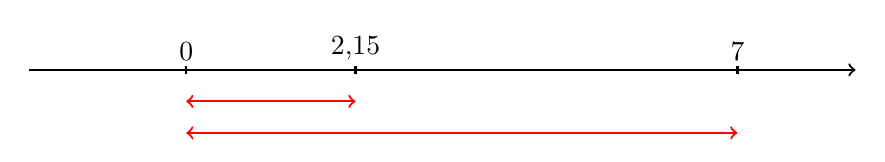
\begin{tikzpicture}
                \draw[->,thick](-2,0)--(8.5,0);
                \draw[-,thick](0,-0.05)--(0,0.05);
                \draw (0,0) node[above]{0};
                \draw[-,thick](2.15,-0.05)--(2.15,0.05);
                \draw (2.15,0) node[above]{2,15};
                \draw[-,thick](7,-0.05)--(7,0.05);
                \draw (7,0) node[above]{7};
                \draw[<->,thick,red](0,-0.4)--(2.15,-0.4);
                \draw[<->,thick,red](0,-0.8)--(7,-0.8);
            \end{tikzpicture}
        \end{center}
        d'où \psshadowbox{$2,15<7$}
        \item Ils sont tous les deux négatifs donc le plus petit est le plus loin de zéro.
        \begin{center}
            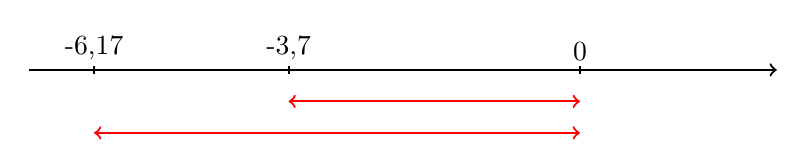
\begin{tikzpicture}
                \draw[->,thick](-7,0)--(2.5,0);
                \draw[-,thick](0,-0.05)--(0,0.05);
                \draw (0,0) node[above]{0};
                \draw[-,thick](-6.17,-0.05)--(-6.17,0.05);
                \draw (-6.17,0) node[above]{-6,17};
                \draw[-,thick](-3.7,-0.05)--(-3.7,0.05);
                \draw (-3.7,0) node[above]{-3,7};
                \draw[<->,thick,red](0,-0.4)--(-3.7,-0.4);
                \draw[<->,thick,red](0,-0.8)--(-6.17,-0.8);
            \end{tikzpicture}
        \end{center}
        d'où \psshadowbox{$-6,17<-3,7$}
        \item L'un est positif et l'autre négatif donc le plus petit est le nombre négatif.
        \begin{center}
            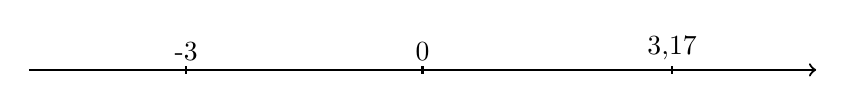
\begin{tikzpicture}
                \draw[->,thick](-5,0)--(5,0);
                \draw[-,thick](0,-0.05)--(0,0.05);
                \draw (0,0) node[above]{0};
                \draw[-,thick](-3,-0.05)--(-3,0.05);
                \draw (-3,0) node[above]{-3};
                \draw[-,thick](3.17,-0.05)--(3.17,0.05);
                \draw (3.17,0) node[above]{3,17};
            \end{tikzpicture}
        \end{center}
        d'où \psshadowbox{$-3<3,17$}
    \end{enumerate}
\end{exemple*1}

\begin{definition}
    \begin{itemize}
        \item L'ordre \textbf{croissant} c'est l'ordre du plus petit au plus grand.
        \item L'ordre \textbf{décroissant} c'est l'ordre du plus grand au plus petit.
    \end{itemize}
\end{definition}

\begin{exemple*1}
    \begin{itemize}
        \item $-3,12$; $-3,09$; $-3,01$; $-2,5$; $-1$; $0$; $12,24$; $12,3$ sont dans l'ordre croissant.
        \item $17,77$; $17,4$; $17,38$; $-1$; $-13$; $-25,7$; $-25,8$; $-31$ sont dans l'ordre d\'ecroissant.
    \end{itemize}
\end{exemple*1}